\documentclass{article}

% if you need to pass options to natbib, use, e.g.:
%     \PassOptionsToPackage{numbers, compress}{natbib}
% before loading neurips_2022


% ready for submission
% \usepackage{neurips_2022}


% to compile a preprint version, e.g., for submission to arXiv, add add the
% [preprint] option:
%     \usepackage[preprint]{neurips_2022}


% to compile a camera-ready version, add the [final] option, e.g.:
\usepackage[final]{neurips_2022}


% to avoid loading the natbib package, add option nonatbib:
%    \usepackage[nonatbib]{neurips_2022}

\usepackage[utf8]{inputenc} % allow utf-8 input
\usepackage[T1]{fontenc}    % use 8-bit T1 fonts
\usepackage{hyperref}       % hyperlinks
\usepackage{url}            % simple URL typesetting
\usepackage{booktabs}       % professional-quality tables
\usepackage{amsfonts}       % blackboard math symbols
\usepackage{nicefrac}       % compact symbols for 1/2, etc.
\usepackage{microtype}      % microtypography
\usepackage{xcolor}         % colors
% \usepackage{ctex}
\usepackage{graphicx}   
\usepackage{wrapfig}
\usepackage{float}
\usepackage{amsmath}
\usepackage{multirow}
\usepackage{multicol}

\bibliographystyle{unsrt}

\title{Playing Aircraft Warfare Game with Reinforcement Learning}

\author{
    Yan Zeng\\
    ShanghaiTech University\\
    \texttt{zengyan@shanghaitech.edu.cn} 
    \AND
    Yijie Fan\\
    ShanghaiTech University\\
    \texttt{fanyj@shanghaitech.edu.cn}\\
    \AND
    Luojia Hu\\
    ShanghaiTech University\\
    \texttt{hulj@shanghaitech.edu.cn}\\
    \AND
    Ziang Li\\
    ShanghaiTech University\\
    \texttt{liza1@shanghaitech.edu.cn}\\
    \AND
    Chongyu Wang\\
    ShanghaiTech University\\
    \texttt{wangchy5@shanghaitech.edu.cn}\\    
}


\begin{document}


\maketitle

% 摘要 分数占比10%s
% \begin{abstract}
    % 摘要没写
% \end{abstract}


\section{Introduction}
\begin{wrapfigure}{H}{7cm}
    \centering
    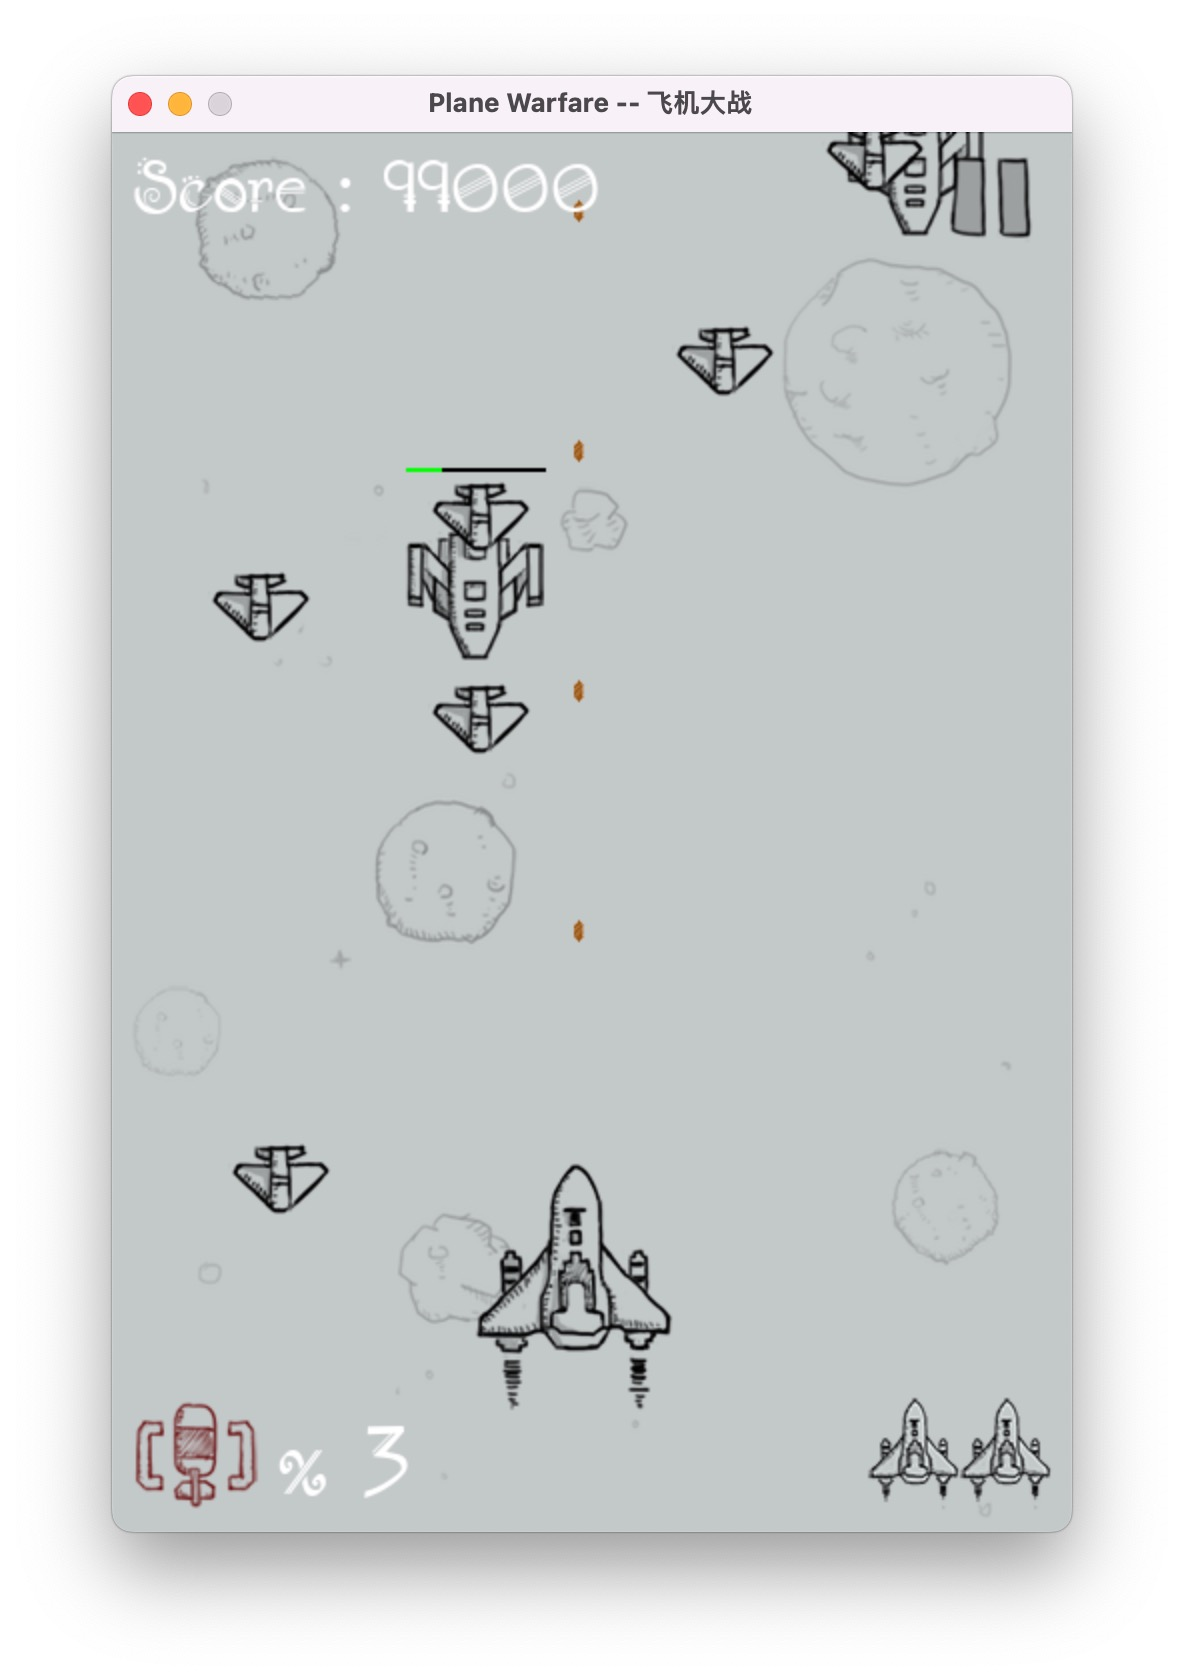
\includegraphics[width=\linewidth]{pictures/game.jpg}
    \caption{The Aircraft Warfare Game}
    \label{fig:aircraft_warfare_game}
\end{wrapfigure}

\par Aircraft Warfare is a classic game we all enjoyed very much, which is also perfect for fully practicing what we have learned in class, as shown in Figure \ref{fig:aircraft_warfare_game}. The rule of the game is rather simple. The \textbf{goal} of the player -- a upward facing aircraft plane -- is to make the score as high as possible. The player can get \textbf{reward} by managing to hit enemies -- downward facing aircraft planes -- with five \textbf{actions}, namely, up, down, left, right, and using the bomb.  The \textbf{state} includes the life value and positions of player and enemies and so on. Game overs when life value decreases to 0.

\par However, playing the game well is quit tough when it comes to difficult mode. Hence we turn to AI for help. To the best of our knowledge, reinforcement learning has shown to be very successful in mastering control policies in lots of tasks such as object recognition and solving physics-based control problems\cite{kempka2016vizdoom}. Specially, Deep Q-Networks (DQN) are proved to be effective in playing games and even could defeat top human Go players\cite{heess2015learning, mnih2013playing}. The reason they can work well is that games can quickly generate large amounts of naturally self-annotated (state-action-reward) data, which are high-quality training material for reinforcement learning. That is, this property of games allows deep reinforcement learning to obtain a large number of samples for training to enhance the effect almost costlessly. For example, DeepMind's achievements such as playing Atari with DQN, AlphaGo defeating Go masters, AlphaZero becoming a self-taught master of Go and Chess. And OpenAI's main research is based on games, such as the progress made in Dota. For these reasons, we believe that training agents based on deep reinforcement learning techniques is a promising solution

\par In this paper, we implement an AI-agent for playing the Aircraft Warfare with Approximate Q-learning method and Deep Q-learning method. For Approximate Q-learning, we extracted four most useful features, i.e., interactions with the closest aircraft, bomb supply, double bullet, and the trade-off between movement and explosion. We trained our agent with an online learning method. For Deep Q-learning, we utilize a convolutional neural network which takes the screen patch as input and outputs the expected converged sum of the discounted reward of taking each action given the current state of the 6 legal actions. We also trained two DQN in case overfitting. 

\par After training for hundreds of episodes, we evaluate our model on the two different tasks. We show that the proposed approximate Q-learning and DQN substantially perform exactly like human beings when in easy mode. In particular, the DQN has the ability to handle very hard mode well in hard mode but still weaker than human player.

% 未完待续
    % In brief, players need to control the plane movement through the up, down, left and right keys on the keyboard, or shoot bullets to destroy the enemy aircrafts (downward facing aircrafts) to obtain points. 

    % Players can obtain points by destroying enemy aircrafts, but they may also be attacked by enemies. When the player's blood volume is 0, the game ends.
    % However, the performance of the player in the game is very complex. Because the aircraft in the game are intelligent, and they will react according to the player's behavior.
    % For example, when the player's plane is close to the enemy plane, the enemy plane will actively launch an attack on the player's plane.

    % In this project, we use this game as our simulation environment, and train the aircraft through the reinforcement learning method to make the aircraft autonomous in the game.

    % \subsection{Aircraft Warfare game settings} 

    % 在这个project中,我们使用了《经典飞机大战》的游戏规则,但是我们对游戏的设置进行了一些修改,以适应我们的强化学习算法。我们采用pygame库来实现游戏的界面,游戏的界面如图\ref{fig:aircraft_warfare_game}所示。

    % In this project, we use the original rules of the `Aircraft Warfare' game, but we make some changes to the game settings to adapt to our reinforcement learning algorithm. We use the pygame library to implement the game interface, as shown in Figure \ref{fig:aircraft_warfare_game}. 

    % % 在游戏中,玩家的飞机会持续发射子弹,玩家可以通过键盘上的上下左右键控制飞机移动。玩家通过空格键发射全屏子弹,能够清空屏幕中出现的所有敌机。但全屏子弹的数量具有限制。

    % In the game, the player's plane will continue to fire bullets, and the player can control the plane movement through the up, down, left and right keys on the keyboard. The player can fire a full-screen bullet through the space key, which can clear all the enemy planes that appear on the screen. But the number of full-screen bullets is limited.

    % % 玩家需要打中敌机来获得分数。

    % % 敌机有三种类型,分别是小型敌机、中型敌机和大型敌机。小型飞机没有血量,打中一次即可消灭。中型和大型飞机都有一定的血量,打中一次会减少一定的血量,当血量为0时消灭。同时,游戏中会有血包和double bullet出现,玩家可以通过接触血包来增加生命数量,通过接触double bullet可以在接下来的一段时间内发射攻击范围更大的双倍子弹。

    % The player needs to hit the enemy plane to get points.

    % There are three types of enemy planes, namely small, medium and large enemy planes. Small enemies can be destroyed by a single bullet hitting. Medium and large enemies have a certain blood volume that hitting once will reduce it, and the enemy will be destroyed when the blood volume is 0. 
    
    % At the same time, there will be blood bags and double bullets appearing in the game. The player can increase the number of lives by touching the blood bag, and can fire double bullets with a larger attack range in the next period of time by touching the double bullet.

\section{ Methodology}
    \subsection{Approximate Q-learning}
        Since the number of states in the Aircraft Warfare Game is extremely large, we choose Approximate Q-learning for reinforcement learning. 
    \subsubsection{Feature Extraction}
        In total, we extracted four features, which are the interaction with the closest aircraft, the interaction with bomb supply, the interaction with double bullet , and the trade-off between movement and explosion. The following will explain in detail how the features are extracted.
        \[Q(s,a) = w_1f_1(s,a)+w_2f_2(s,a)+w_3f_3(s,a)+w_4f_4(s,a)\]
    
        In this game, it is very necessary to control the distance between our aircraft and enemy aircraft and props.Thus,we use the Manhattan distance to measure the interaction of the aircraft with the external environment. For the current state $s$, we observe the location of the nearest enemies, game props to the aircraft. Next, we analyze the effect of action $a$ on the Manhattan distance between the aircraft and the aforementioned target. The weights corresponding to each of these features reflect the choices and trade-offs made by the aircraft in various situations.The purpose of the plane's actions can be highly summarized as attacking, dodging, and picking up props. Both affect the value of $Q(s,a)$ and the training of Approximate Q-learning.
    \subsubsection{Training}
        In the training phase, we train the learning with multiple hyperparameters and update the weights according to the formula below.
        \[ \mathrm{difference} = r+\gamma \mathop{\mathrm{max}}_{\alpha'}Q(s',a')-Q(s,a)\]
        \[ Q(s,a) \xleftarrow{} Q(s,a) +\alpha[\mathrm{difference}]\]
        \[w_i \xleftarrow{} w_i+\alpha[\mathrm{difference}] f_i(s,a)\]
        Our training is an online learning approach. After getting a new state $s$ in each round, we choose the action $a$ with the highest $Q(s,a)$. After taking the action in the current round, we get state $s$. Then, we use these two states with association to obtain the difference and update the parameters of the model. $\gamma$ is the discount parameter.$\alpha$ is the learning rate. The adjustment of these two parameters can better help our model to converge.
        
        % % 在这个project中,我们会使用approximate q-learning 来训练aircraft玩游戏。
    
        % We will use an approximate Q-learning to train the aircraft to play the game. The approximate Q-learning algorithm is a model-free reinforcement learning algorithm, which uses a weighted sum of features to approximate the Q function. It is suitable when the state space is large. 
    
        % \subsection{Features and Reward function}
    
        % The features consists of mainly the position of the aircraft, enemies, and bouns (double bullet and additional life). In addition, the current status including the score, the life number remaining are also used. We will take a weighted sum of these features as the current state.
    
        % % \subsection{Reward function}
    
        % \subsection{Action}
    \subsection{Deep Q Network}
    % DQN属于DRL(深度强化学习)的一种,它是深度学习与Q学习的结合体。前面讲了采用S-A表格的局限性,当状态和行为的组合不可穷尽时,就无法通过查表的方式选取最优的Action了。这时候就该想到深度学习了,想通过深度学习找到最优解在很多情况下确实不太靠谱,但是找到一个无限逼近最优解的次优解,倒是没有问题的。
    % 因此DQN实际上,总体思路还是用的Q学习的思路,不过对于给定状态选取哪个动作所能得到的Q值,却是由一个深度神经网络来计算的了
    Deep Q Network is a kind of Deep Reinforcement Learning, which is a combination of Deep Learning and Q-learning. Due to the limitations of Q-learning that it is impossible to choose the best action when the number of combinations of states and actions is infinite, using a deep neural network to help determine the action is reasonable. 
    
    \subsubsection{DQN algorithm} In the Aircraft Warfare Game the environment is deterministic, so all the equations listed below are formulated deterministically for simplicity. Our aim will be to train a policy that can maximize the cumulative, discounted reward $R_{t_0} = \sum_{t=t_0}^{\infty} {\gamma}^{t-t_0}r_t$,here the $\gamma$ is the discount factor,which should be a constant between 0 and 1 to make sure the sum can converge.In the Q-learning algorithm, we get a table of the $Q$ values of the combinations of states and actions, then we construct a policy that maximizes the rewards:
    $$\pi^*(s) = \arg\!\max_a \ Q^*(s, a)$$
    However, since the number of the combinations of states and actions is infinite in this scene, so we use a neural network to resemble $Q^*$. And by Bellman equation,we get:
    $$Q^{\pi}(s, a) = r + \gamma Q^{\pi}(s', \pi(s'))$$
    The difference between the two sides of the equation is known as the difference discussed in the lecture:
    $$\delta = Q(s, a) - (r + \gamma \max_{a'} Q(s', a'))$$
    To minimize this difference, we use the Huber loss which acts
    like the mean squared error when the error is small, but like the mean
    absolute error when the error is large - this makes it more robust to
    outliers when the estimates of $Q$ are very noisy. We calculate
    this over a batch of transitions, $B$, sampled from the replay
    memory:
    $$\mathcal{L} = \frac{1}{|B|}\sum_{(s, a, s', r) \ \in \ B} \mathcal{L}(\delta)$$
    
    $$\text{where} \quad \mathcal{L}(\delta) = \begin{cases}
         \frac{1}{2}{\delta^2}  & \text{for } |\delta| \le 1, \\
         |\delta| - \frac{1}{2} & \text{otherwise.}
       \end{cases}$$
    \subsubsection{DQN Structure and Training}
    We first tried  a convolutional neural network which takes the screen patch as input and outputs the expected converged sum of the discounted reward of taking each action given the current state of the 6 legal actions. To prevent overfitting, we trained two Deep Q Networks: policy network and target network. They have the same structure but the parameters are different. We get the best action from the policy network and computes the $\max_{a'} Q(s', a')$ from the target network for added stability. To explore the environment, we use the $\epsilon$ greedy method when choosing the action and the value of $\epsilon$ is decayed with time to lower the regret. However, the result of using the convolutional neural network is not satisfying after we trained it for 600 episodes. The reason for this is that the convolutional neural net combines feature extractor and learning together, so some useless features might be considered by the net.
    
    To solve this problem, we decided to extract the features by ourselves. We mainly considered the position of the plane, the relative position between the nearest enemy and the plane, the type of the nearest enemy, the relative position between the prop and the plane, life number remained, bomb number remained and whether the plane has been strengthened. After training of 600 episodes, we got a satisfying result.
\section{Result}
To evaluate the performance of Approximate Q-learning and DQN, we first considered the goal of playing this game which is to maximize the score. Therefore, we choose score as our evaluation method. The scores are listed below:
\begin{table*}[h]
	\centering
	\begin{tabular}{ccc}
		\specialrule{.16em}{0pt} {.65ex}
		Method & Highest Score  & Average Score \\
		\midrule
		  Approximate Q-learning & 1,324,000  & 886,000\\
		  DQN &  1,557,000  & 1,127,000\\
            Human (group member) & 673,000 & 425,000\\
		\specialrule{.16em}{.4ex}{0pt}
	\end{tabular}
	\caption{The highest and average score after training}
 	\label{tab:osdi}
\end{table*}

From these tables, we can find that both Approximate Q-learning and DQN have outperformed our group member in this game, which implies that both methods have achieved satisfying results.
To better evaluate the performance of these two methods, we modified the game environment and added a Hard Mode in which the enemies move faster and the number of enemies in the screen becomes larger. The result of Hard Mode is listed below:
\begin{table*}[h]
	\centering
	\label{tab:osdi}
	\begin{tabular}{ccc}
		\specialrule{.16em}{0pt} {.65ex}
		Method & Highest Score  & Average Score \\
		\midrule
		  Approximate Q-learning & 1,324,000  & 886,000\\
		  DQN &  1,557,000  & 1,127,000\\
            Human (group member) & 673,000 & 425,000\\
		\specialrule{.16em}{.4ex}{0pt}
	\end{tabular}
    \caption{Hard Mode Result}
 	\label{tab:osdi}
\end{table*}

From the viewpoint of human, the keys to maximize the score are getting close to the enemies when the plane can shoot the enemies, getting far away from the enemies when the plane is too close to the enemies and can't shoot the enemies, getting the props when needed. From the process of the AI playing the game, both Approximate Q-learning and DQN have learned these keys. However, the actions taken by the Approximate Q-learning are sometimes very noisy, for example it might frequently take left and right actions when the enemy is in front.

\section{Conclusion}
\par In this paper, we presented a complete architecture for playing the Aircraft Warfare. We modified the open source code of Aircraft Wars to extract state and further get features that could be learned by our model. We implemented a model based on approximate Q-learning and trained it using online training method. The performance of the model is quite outstanding. It can both control the distance between our aircraft and enemies and hit the enemies from a relative far distance. To further improve its performance and learn more high-level information, we implements an model with DQN. In easy mode, both approximate Q-learning and deep Q-learning performs just like human beings. And DQN even has a better highest score than human player. That is the DQN model can handle tricky scenarios much better. In hard mode, both are still able to perform  near human level. In this project, we used only an external game framework to implement a Q-based model from scratch, taking full advantage of what we learned in class. During this period, we encountered many difficulties, but we solved them one by one and finally achieved satisfactory results.
% 

\newpage
{
\small
\bibliography{neurips_2022}
}

\appendix



\end{document}